\documentclass{beamer}
\usetheme{Darmstadt}
\usecolortheme{beaver}
\usepackage{booktabs}
\usepackage{hyperref}

\usepackage[utf8]{inputenc}
\usepackage{graphicx}
\graphicspath{ {./images/} }

%Information to be included in the title page:
\title{Sample title}
\author{Brandon Hosley}
\institute{University of Illinois - Springfield}
\date{\today}

\begin{document}
\frame{\titlepage}

\begin{frame}{Overview}
\tableofcontents
\end{frame}

\section[Q1.1]{Q1A: What is a Na\"{i}ve-Bayes classifier?}

\begin{frame}{Sample frame title}
\begin{block}{Remark}
	Sample text
\end{block}

\begin{alertblock}{Important theorem}
	Sample text in red box
\end{alertblock}

\begin{examples}
	Sample text in green box. The title of the block is ``Examples".
\end{examples}

\end{frame}

\section[Q1.2]{Q1B: What are the evaluation metrics for classification in machine learning?}

\section[Q2]{Q2: Hastie and Tibshirani Summary}

\begin{frame}{Tibshirani Lecture: Classification}
\begin{itemize}
	\item<1-> Linear Regression
	\begin{itemize}
		\item<1-> Simple approximation method
		\item<1-> Great for estimating slope of data
		\item<1-> From this one may generate confidence interval
	\end{itemize}
	\item<2> Hypothesis Testing
	\begin{itemize}
		\item<2> Testing against a null hypothesis
		\item<2>[] $H_0$ : No relationship between $X$ and $Y$.
		\item<2> Testing for the probability of independent variable distribution 
	\end{itemize}
\end{itemize}
\only<1>{\includegraphics[width=0.75\linewidth]{ConfidenceIntervals}}
\only<2>{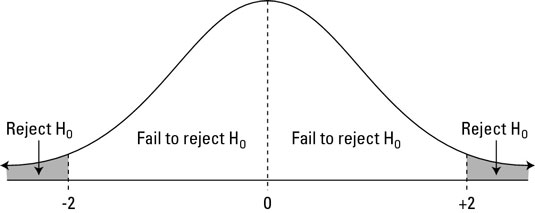
\includegraphics[width=0.75\linewidth]{nullHypothesis}}
\end{frame}

\end{document}
